\documentclass{article}

% Language setting
% Replace `english' with e.g. `spanish' to change the document language
\usepackage[english]{babel}

% Set page size and margins
% Replace `letterpaper' with `a4paper' for UK/EU standard size
\usepackage[letterpaper,top=2cm,bottom=2cm,left=3cm,right=3cm,marginparwidth=1.75cm]{geometry}

% Useful packages
\usepackage{amsmath}
\usepackage{graphicx} % Required for including images
\usepackage{cite}     % Required for handling citations
\usepackage[colorlinks=true, allcolors=blue]{hyperref}

\usepackage{listings}
\usepackage{xcolor}

% Define colors for syntax highlighting
\definecolor{keywordcolor}{RGB}{0,0,255}
\definecolor{commentcolor}{RGB}{0,128,0}
\definecolor{stringcolor}{RGB}{255,0,0}

% Set the style for C++ code
\lstdefinestyle{cppstyle}{
	language=C++,
	keywordstyle=\color{keywordcolor},
	commentstyle=\color{commentcolor},
	stringstyle=\color{stringcolor},
	basicstyle=\ttfamily,
	numbers=left,
	numberstyle=\tiny,
	stepnumber=1,
	numbersep=5pt,
	frame=single,
	tabsize=4,
	breaklines=true
}


\title{Self Balancing Robot}
\author{Muhammad Haris Mujeeb}

\begin{document}
\maketitle

\begin{abstract}
This report focuses on the design of a Two-wheeled Self-Balancing Robot, which embodies the classic inverted pendulum problem. Using a Kalman filter for MPU6050 sensor data fusion and implementing PID controllers. This project aims to develop a robust two-wheeled self-balancing robot that can be observed and controlled remotely. The coding for the Arduino Nano has been executed using \href{https://platformio.org/}{PlatformIO}, with the complete project available on this \href{https://github.com/haris-mujeeb/Self-Balancing-Robot}{GitHub repository}.
\end{abstract}

\section{Introduction}
Two-wheeled vehicles are generally more agile, allowing easier navigation through tight spaces, making them ideal for congested environments. Their lighter weight and compact size facilitate easier handling while also enhancing energy efficiency. In addition, they are typically less expensive to purchase and maintain, increasing accessibility for a wider range of users.
A good base model to build such robot is \href{https://www.elegoo.com/products/elegoo-tumbller-self-balancing-robot-car}{ELEGOO Tumbler} (shown in Fig. \ref{fig:tumbler}), which provided nearly all the hardware required as a DIY kit.

\begin{figure}[h]
    \centering
    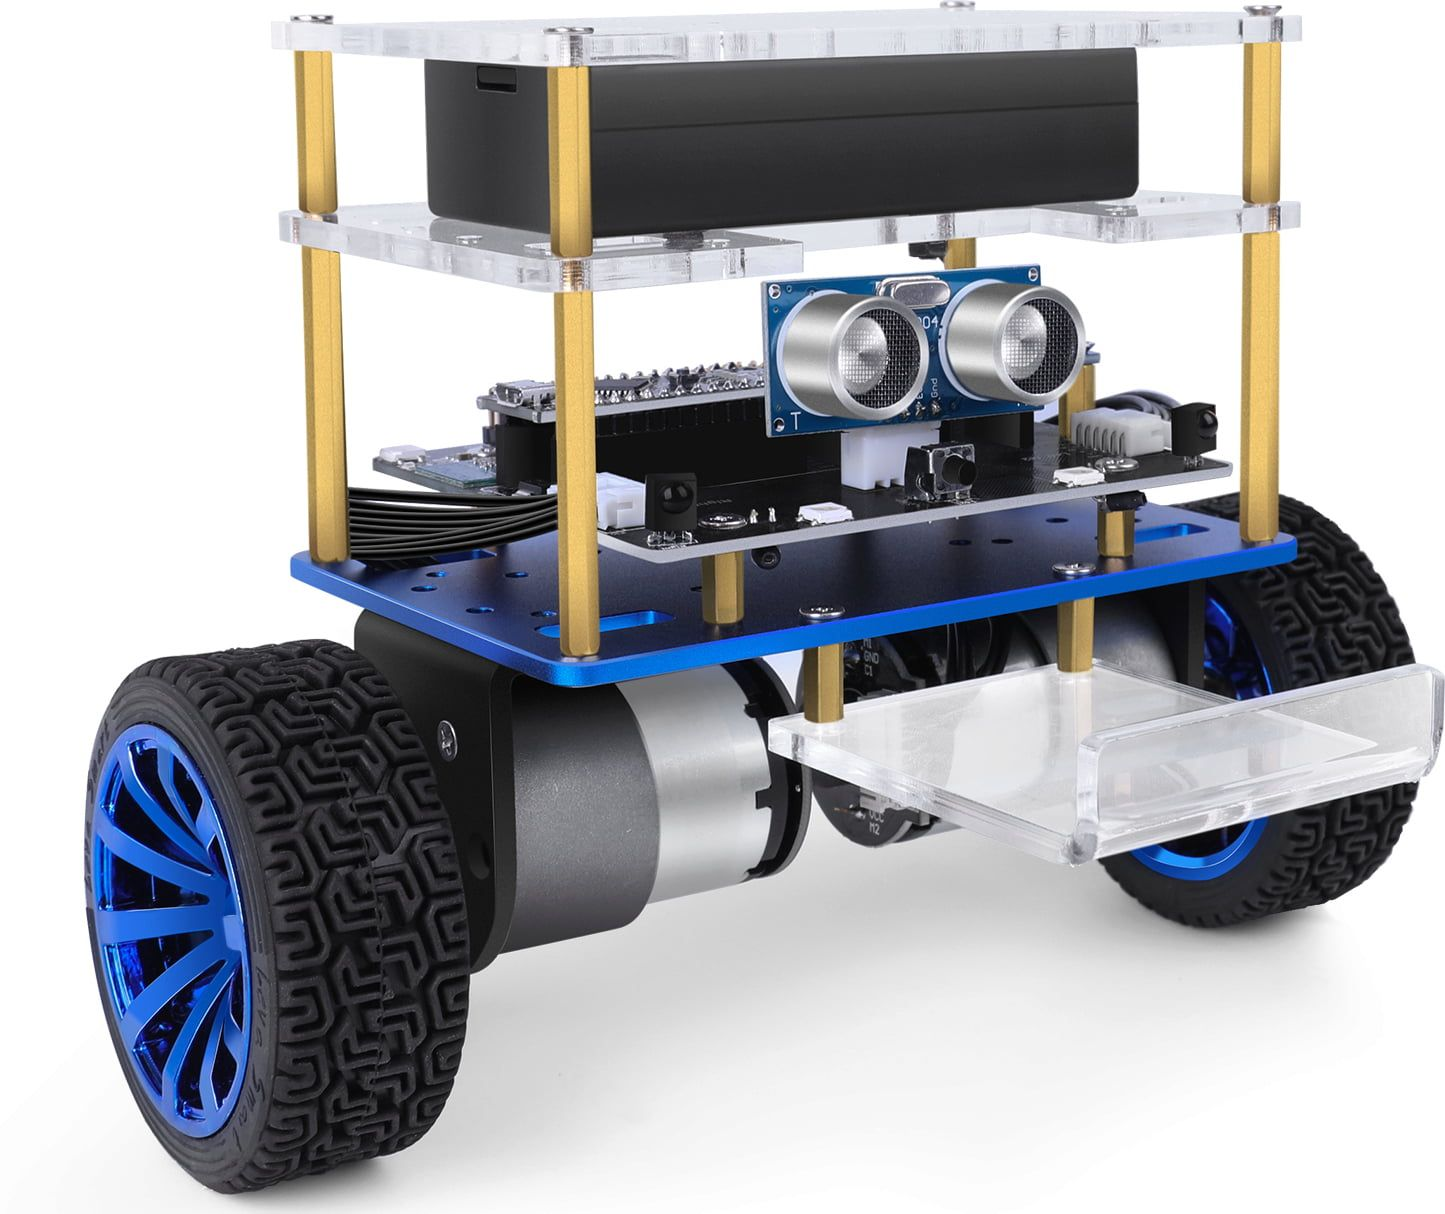
\includegraphics[width=0.25\linewidth]{assets/tumbler.jpg}
    \caption{\label{fig:tumbler} ELEGOO Tumbler which was used for this project \cite{elegoo}.}
\end{figure}

\section{Hardware}

\subsection{ATmega328P}
The ATmega328P is a popular microcontroller from Microchip Technology, widely used in embedded systems and electronics projects. It belongs to the AVR family of microcontrollers and is renowned for its versatility, ease of use, and robust performance (shown in Fig. \ref{fig:ATmega328p}). Its most significant benefits is its abundance of resources and community support, particularly due to its compatibility with the Arduino platform. With a 16 MHz clock speed, 32 KB of flash memory, 2 KB of SRAM, and 1 KB of EEPROM, the ATmega328P provides ample resources for this projects application. 

\begin{figure}[h]
    \centering
    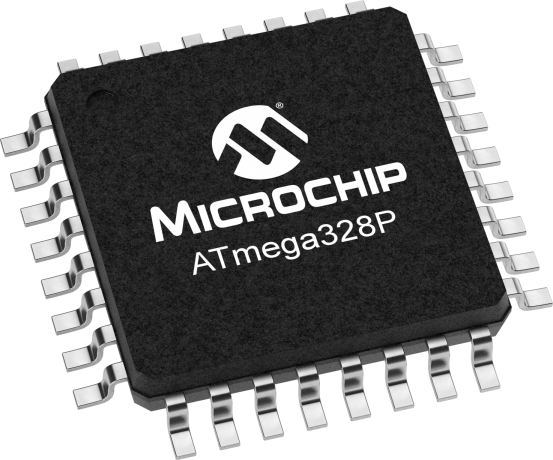
\includegraphics[width=0.15\linewidth]{assets/ATmega328p.png}
    \caption{ATMEGA328P ANR \cite{atmega_microchip}.}
    \label{fig:ATmega328p}
\end{figure}

\subsection{MPU6050}
The MPU6050 is a widely used sensor that integrates a three-axis gyroscope and a three-axis accelerometer on a single chip, making it essential for motion tracking and stabilization applications (shown in Fig. \ref{fig:mpu-6050}). Its compact design and built-in Digital Motion Processor (DMP) enable real-time processing of sensor data, which is crucial for robotics, drones, and wearable devices.
In applications like self-balancing robots, it provides accurate orientation and acceleration data necessary for maintaining stability. 

\begin{figure}[h]
    \centering
    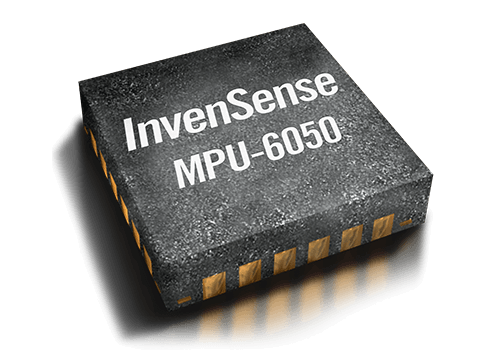
\includegraphics[width=0.15\linewidth]{assets/mpu-6050.png}
    \caption{MPU-6050 \cite{mpu6050}.}
    \label{fig:mpu-6050}
\end{figure}


\subsection{TB6612FNG H-bridge}
The TB6612FNG H-bridge \cite{TB6612FNG} together with SN74LVC2G14 schmitt-trigger \cite{SN74LVC2G14} provide a powerful and reliable motor control solution for self-balancing robots. This combination allows for precise motor operation, enabling the robot to adapt quickly to its environment and maintain stability effectively.

\subsection{Geared DC Motors}
37mm High Torque 12V Gearbox DC Motors with Speed Encoders were used in this project. Multiple manufacurer are producing these kind of motors (shown in Fig. \ref{fig:dc-motors}). Motors from NHYTech were in this case.

\begin{figure}[h]
    \centering
    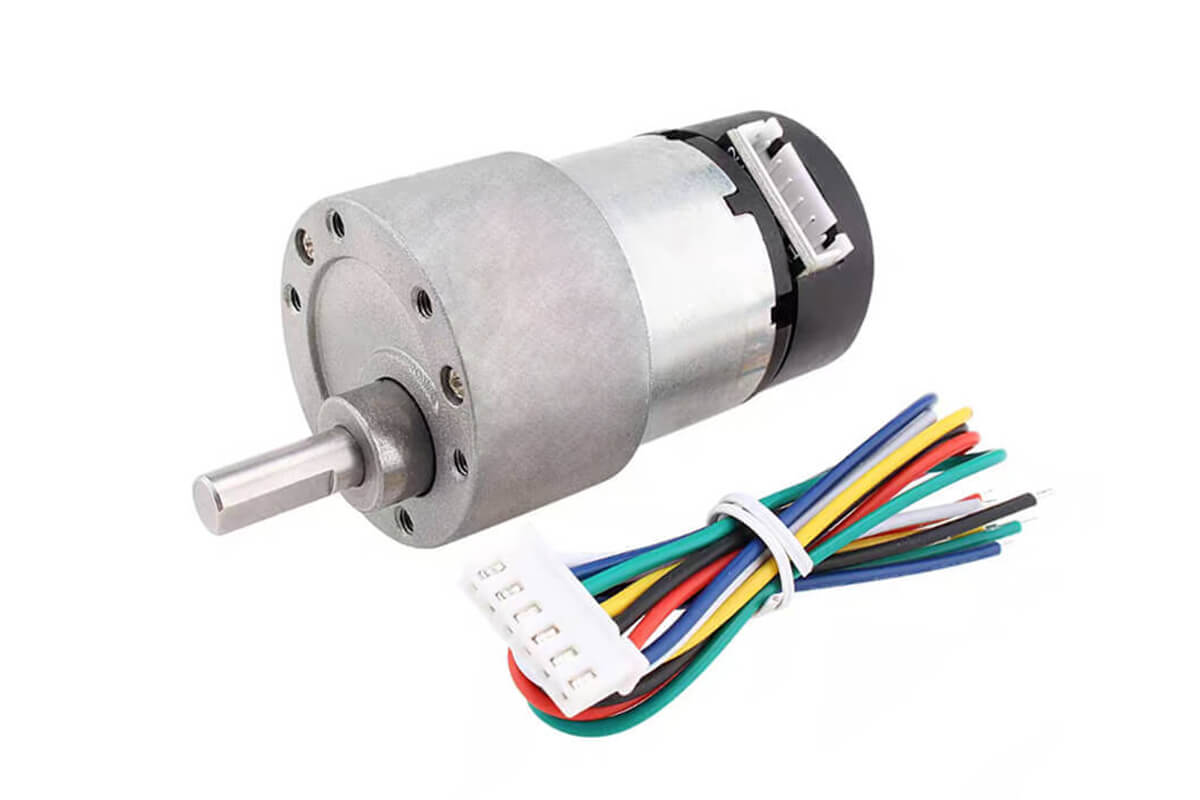
\includegraphics[width=0.25\linewidth]{assets/dc-motor-with-encoder.jpg}
    \caption{Similar construction motors were used in this project \cite{dc-motor}.}
    \label{fig:dc-motors}
\end{figure}



\section{Mathematical Modelling}
$$
\begin{bmatrix}
    \dot{x} \\
    \ddot{x} \\
    \dot{\psi} \\
    \ddot{\psi}
\end{bmatrix}
= A
\begin{bmatrix}
    x \\
    \dot{x} \\
    \psi \\
    \dot{\psi}
\end{bmatrix}
+ B u_{input}
$$


\subsection{Extended Kalman Filter (EKF)}
The Kalman filter (KF) provides a more sophisticated approach, estimating the true state of the system by minimizing the mean of the squared error. It involves prediction and update steps. However,  assumes that both the process and measurement models are linear. However, many real-world systems, such as robotic motion and sensor fusion, exhibit inherent nonlinearities. When linearization is not feasible, the standard KF becomes inaccurate. 

To address this limitation, the Extended Kalman Filter (EKF) extends the KF to nonlinear systems by employing a first-order Taylor series expansion. This method approximates the nonlinear system dynamics and measurement models with locally linearized representations, allowing the filter to be applied in scenarios where exact linearization is not feasible.

The EKF is an extension of the Kalman Filter for nonlinear systems, utilizing first-order Taylor series expansion to linearize process and measurement models. EKF maintains a Gaussian belief over the state, updating it through a prediction-correction cycle. The Jacobian matrices of the system dynamics and measurement functions are used to approximate state transitions and measurement updates. Its advantages include handling nonlinearities, fusing multi-sensor data, and improving estimation accuracy in noisy environments. 

\subsubsection{General State Equation}
For non-linear system, with Stochastic disturbances:
\begin{equation}
\begin{aligned}
	\dot{\underline{x}}(t) &= f\left( \underline{x}(t), \underline{u}(t) \right) + \underline{d}(t) \\
	\underline{y}(t) &= h\left( \underline{x}(t) \right) + \underline{n}(t)
\end{aligned}
\end{equation}
where,
\begin{itemize}
	\item $ \dot{\underline{x}}(t) $: This represents the time derivative of the state vector $ \underline{x}(t) $, indicating how the state evolves over time.
	\item $ f $: This is a nonlinear function that describes the system dynamics, taking the current state $ \underline{x}(t) $ and the control input $ \underline{u}(t) $ as arguments. It captures how the state changes based on the current state and control inputs.
	\item $ \underline{d}(t) $: This term represents stochastic disturbances (or process noise) affecting the state dynamics, typically modeled as a zero-mean Gaussian noise.
	\item $ y(t) $: This is the measurement vector at time $ t $, representing the observed outputs of the system. It is the data collected from sensors or measurement devices.
	\item $ h $: This is a nonlinear measurement function that maps the true state vector $ \underline{x}(t) $ to the measurement space. It describes how the state influences the measurements. The function $ h $ can be complex and may involve various transformations of the state variables.
	\item $ n(t) $: This term represents measurement noise, which is also typically modeled as zero-mean Gaussian noise. It accounts for inaccuracies in the measurements due to sensor errors, environmental conditions, or other random factors that can affect the observed data.
\end{itemize}

\subsubsection{State Estimation}
For a non-linear system the state form is as follows,
\begin{equation}
\begin{aligned}
	\dot{\hat{\underline{x}}}(t) &= f\left( \underline{\hat{x}}(t), \underline{u}(t) \right) + \underline{K}\left( y(t) - \hat{y}(t) \right) \\
	\hat{y}(t) &= h\left( \underline{\hat{x}}(t) \right)  \label{eq:eq}
\end{aligned}
\end{equation}
The Kalman gain $\underline{K}$ is computed to optimally balance estimation uncertainty and measurement noise. To achieve this, the system is first linearized around the current state estimate by computing the Jacobians of the process and measurement models. To linearize the system around the current state estimate, the Jacobian matrices, which represent the first-order partial derivatives of the nonlinear functions, are computed as follows:
\begin{equation}
\underline{A}(t) = \frac{\mathrm{d}f}{\mathrm{d}\underline{x}} \bigg|_{\underline{\hat{x}}(t), \underline{u}(t)} \quad \text{and} \quad
\underline{C}(t) = \frac{\mathrm{d}h}{\mathrm{d}\underline{x}} \bigg|_{\underline{\hat{x}}(t)}  \label{eq:eq}
\end{equation}
where $\underline{A}(t)$ represents the partial derivatives of the state dynamics function $f$ and $\underline{C}(t)$ represents the partial derivatives of the measurement function $h$.
\begin{figure}[h]
	\centering
	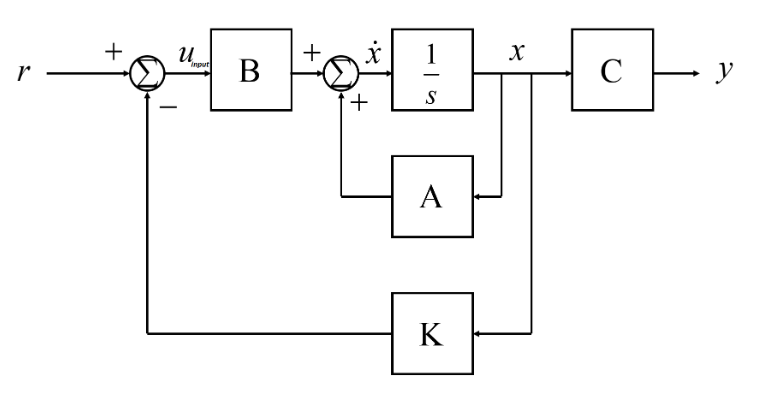
\includegraphics[height=5cm]{assets/block_representation_kalman_filter.png}
	\caption{Block representation of state space system showing the system matrices $A$, $B$ and $C$ as well as the gain matrix $K$.}
	\label{fig:block_representation_kalman_filter}
\end{figure}
\subsubsection{Covraince Matrix}
The evolution of the state estimation covariance matrix follows the continuous-time Riccati equation, given by:
\begin{equation}
\dot{P}(t) = \underline{A}(t) P(t) + P(t) \underline{A}^T(t) + Q - P(t) \underline{C}^T(t) R^{-1} \underline{C}(t) P(t)  \label{eq:eq}
\end{equation}
Where, 
\begin{itemize}
	\item $\dot{P}(t)$: his represents the time derivative of the covariance matrix $\dot{P}(t)$, which quantifies the uncertainty in the state estimate over time.
	\item $\underline{A}(t)$: This is the state transition matrix, which describes how the state evolves from one time step to the next.
	\item $Q$: This is the process noise covariance matrix, representing the uncertainty in the process model.
	\item $\underline{C}(t)$: This is the measurement matrix, which relates the state to the measurements.
	\item $R$: This is the measurement noise covariance matrix, representing the uncertainty in the measurements.
\end{itemize}
The Kalman filter is initialized with an initial covariance matrix:
\begin{equation}
	P(0) = \mathbf{E}(\Delta\underline{x}(0) \Delta\underline{x}^T(0))  \label{eq:eq}
\end{equation}
The optimal Kalman gain, balancing estimation uncertainty and measurement noise, is given by:

\begin{equation} \underline{K}(t) = P(t) \underline{C}^T R^{-1} \end{equation}
The time-discrete Kalman filter state update equations are:
\begin{equation}
	\begin{aligned}
		\underline{x}_{k} &= \underline{A} \underline{x}_{k-1} + \underline{B} \underline{u}_{k} + \underline{d}_{k-1} \\
		\underline{y}_{k} &= \underline{C} \underline{x}_{k} + \underline{n}_{k}  \label{eq:eq}
	\end{aligned}
\end{equation}
where $\underline{x}_k$ is the state vector, $\underline{B}$ the control input matrix, and $\underline{y}_k$ the measurement vector. The discrete state-space representation is:
\begin{equation}
	\begin{aligned}
		\underline{\dot{x}}(t) = \underline{A}.\underline{x}(t) + \underline{B}.\underline{u}(t) \\
		\underline{y}(t) = \underline{C}.\underline{x}(t) + \underline{D}.\underline{u}(t)  \label{eq:eq}
	\end{aligned}
\end{equation}
The state covariance matrix is:
\begin{equation}
	\mathbf{P}_k = \begin{bmatrix} P_{00} & P_{01} \\ P_{10} & P_{11} \end{bmatrix}  \label{eq:eq}
\end{equation}
where $P_{00}$ represents uncertainty in the angle estimate and $P_{11}$ in gyroscope bias. The Kalman gain is computed as:
\begin{equation}
	\begin{aligned}
		\underline{K}_{k} &= \underline{P}_{k}^- \ \underline{C}^T ( \underline{C} \ \underline{P}_{k}^-\ \underline{C}^T  +\underline{R})^{-1} \\ \\
		\mathbf{K}_k &= \begin{bmatrix} \frac{ P_{00} }{ P_{00}  
				+ R_{angle}} \\ \frac{ P_{10} }{ P_{00}  
				+ R_{angle}} \end{bmatrix}
	\end{aligned}  \label{eq:eq}
\end{equation}
Following the prediction step, the measurement update step refines the state estimate using the Kalman gain, which is derived to minimize the posterior estimation error covariance (see Appendix \ref{appendix:B} for detailed calculations):
\begin{equation}
	\begin{aligned}
		\underline{P}_{k} &= \ (\underline{I} - \underline{K}_{k} \ \underline{C}) \ \underline{P}_{k}^- \label{eq:eq}
	\end{aligned}
\end{equation}


\subsection{Software Implementation of EKF}
For the implementation of the Extended Kalman Filter (EKF), we utilized the Kalman filter library developed by Kristian Lauszus~\cite{github_kalman_filter}. This library was modified in accordance with the GNU General Public License to meet the specific requirements of our project.
\begin{lstlisting}[style=cppstyle2]
#include <Arduino.h>

class KalmanFilter {
 private:
  float m_dt, m_Q_angle, m_Q_gyro, m_R_angle, m_C_0;
  float q_bias = 0, angle_err = 0;
  float P[2][2] = {{1, 0}, {0, 1}}; // Covariance matrix
  float K_0 = 0, K_1 = 0;

 public:
  float angle = 0;

KalmanFilter(float dt, float Q_angle, float Q_gyro, float R_angle, float C_0)
: m_dt(dt), m_Q_angle(Q_angle), m_Q_gyro(Q_gyro), m_R_angle(R_angle), m_C_0(C_0) {}

float getAngle(float measured_angle, float measured_gyro) {
	// Predict
	angle += (measured_gyro - q_bias) * m_dt;
	angle_err = measured_angle - angle;
	
	// Update covariance matrix
	P[0][0] += m_Q_angle - P[0][1] - P[1][0];
	P[0][1] -= P[1][1];
	P[1][0] -= P[1][1];
	P[1][1] += m_Q_gyro;
	
	// Compute Kalman gain
	float E = m_R_angle + m_C_0 * P[0][0];
	K_0 = (m_C_0 * P[0][0]) / E;
	K_1 = (m_C_0 * P[1][0]) / E;
	
	// Update state
	angle += K_0 * angle_err;
	q_bias += K_1 * angle_err;
	
	// Update covariance matrix
	float C0_P00 = m_C_0 * P[0][0];
	P[0][0] -= K_0 * C0_P00;
	P[0][1] -= K_0 * P[0][1];
	P[1][0] -= K_1 * P[0][0];
	P[1][1] -= K_1 * P[0][1];
	
		return angle;
	}
};
\end{lstlisting}

\section{Cascaded PID Control Loop}

The algorithm utilizes cascade Proportional–Integral–Derivative (PID) control loop to maintain balance and control the robot's movement in real time. The balancing is achieved by continuously monitoring and adjusting its state using sensor feedback. The key sensor inputs include the robot's pitch angle, gyro data and motor's encoder values, which provide information on the robot's orientation, angular velocities and position.The algorithm utilizes cascade PID control loops to maintain balance and control the robot's movement in real time. The approach includes computing control outputs for pitch, yaw, and position periodically, which are then used to adjust the motor speeds by sending corresponding pulse-width-modulation (PWM) signals to the motor driver (see Fig. \ref{fig:control-loop}).

\begin{figure}[h]
	\centering
	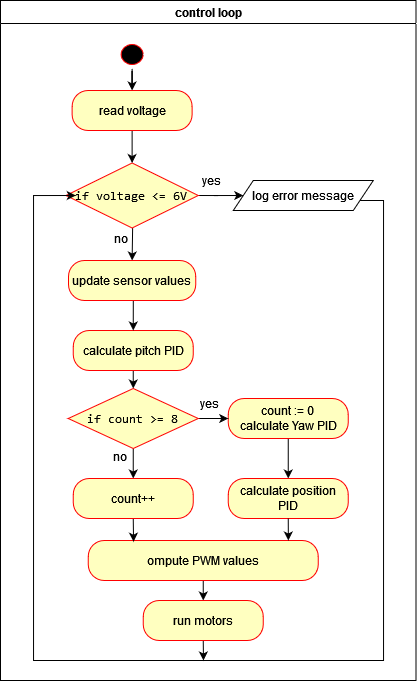
\includegraphics[width=0.5\linewidth]{assets/Control_Loop.png}
	\caption{A simplified block diagram of the control loop. }
	\label{fig:control-loop}
\end{figure}

As the pitch angle is more important for system stability, therefore it is updated more frequently (e.g. updated every cycle), while the PID output values for the yaw angle and position control are updated longer duration of time (e.g. after every 8th cycle).

\subsection{Basic PID Structure}
The PID controller output can be expressed mathematically as:

\begin{equation}
	u(t) = K_p e(t) + K_i \int_0^t e(\tau)d\tau + K_d \frac{d}{dt}e(t)
\end{equation}

Where:
\begin{itemize}
	\item $u(t)$ is the control signal
	\item $e(t)$ is the error signal
	\item $K_p$ is the proportional gain
	\item $K_i$ is the integral gain
	\item $K_d$ is the derivative gain
\end{itemize}



\subsection{Position Control Loop}
The outer loop manages the robot's position:

\begin{equation}
	\theta_{desired} = K_{px}(x_{desired} - x_{measured}) + K_{dx}\frac{d}{dt}(x_{desired} - x_{measured})
\end{equation}


\section{Implementation Considerations}
\subsection{Discrete Time Implementation}
For digital implementation, the PID controller is discretized:

\begin{equation}
	u[n] = K_p e[n] + K_i T_s \sum_{k=0}^n e[k] + K_d \frac{e[n] - e[n-1]}{T_s}
\end{equation}

Where $T_s$ is the sampling period.


\section{Tuning Methodology}
For tuning a general combination of Ziegler-Nichols method and practical tuning guidelines were used.
\subsection{Ziegler-Nichols Method}
The Ziegler-Nichols tuning method follows these steps:
\begin{enumerate}
	\item Set $K_i$ and $K_d$ to zero
	\item Increase $K_p$ until system oscillates with period $T_u$
	\item Record the ultimate gain $K_u$
	\item Calculate parameters:
	\begin{align*}
		K_p &= 0.6K_u \\
		T_i &= 0.5T_u \\
		T_d &= 0.125T_u
	\end{align*}
\end{enumerate}

\subsection{Practical Tuning Guidelines}
The general tuning guidelines are as follows:

\begin{itemize}
	\item Begin with small $K_p$ (= 10)
	\item Add derivative term ($K_d = 0.1K_p$)
	\item Fine-tune until stable
\end{itemize}


\subsection{Pitch PID Control:}
The pitch control loop ensures the robot maintains its upright position. The primary objective of the pitch controller is to minimize the deviation of the robot's pitch angle from a set-point, which is ideally zero degrees (i.e., upright). The pitch control output is calculated using the PD algorithm, where the error is the difference between the current pitch angle and the desired pitch angle. 
\begin{equation}
	\tau_{\theta,pid} = K_{p\theta}({\theta_{desired} - \theta_{measured}}) + K_{d\theta}\frac{d}{dt}(\theta_{desired} - \theta_{measured})
\end{equation}

Below is its code implementation:
\begin{lstlisting}[style=cppstyle]
inline void runPitchControl() {
	// Compute balance control output
	pitch_pid_output = kp_balance * (kalman.angle - 0) 
	+ kd_balance * (gyro_x  - 0);
}
\end{lstlisting}

\begin{itemize}
	\item \textbf{Proportional (P):} The proportional term is based on the current error (the pitch angle deviation from the desired value). A higher proportional gain causes the robot to respond more aggressively to larger deviations.
	\item \textbf{Derivative (D):} The derivative term anticipates future errors by considering the rate of change of the error (pitch angular velocity deviation from desired value). It provides a damping effect, which helps to reduce overshooting and oscillations.
	\item \textbf{Integral (I):} Because the system is inherently unstable when at desired upright position (steady state error can never be zero) thus adding the integral term is unnecessary. 
	
\end{itemize}

The output of the pitch PD controller ($\text{pitch\_pid\_output}$) is then used to adjust the robot's motor speeds to counteract any tilting or imbalance.

\subsection{Yaw Control:}
Yaw control is responsible for controlling the robot's rotational movement around its vertical axis. The yaw PID controller computes the control output based on the robot's angular velocity, which is measured by the gyroscope along the z-axis. The yaw control adjusts the motor speeds to achieve the desired rotational velocity, ensuring the robot maintains a stable heading.
\begin{equation}
	\tau_{\phi,pid} = K_{d\phi}\frac{d}{dt}(\phi_{desired} - \phi_{measured})
\end{equation}


Below is its code implementation:
\begin{lstlisting}[style=cppstyle]
inline void runYawControl(){
	yaw_pid_output = kd_turn * gyro_z;
}
\end{lstlisting}

Similar to pitch control, the yaw controller follows the PID principles:
\begin{itemize}
	\item \textbf{Proportional (P):} In order to calculate yaw angle, a high computational overhead is required, while yaw angle is not critical for balancing thus the proportional term is ignored.
	\item \textbf{Integral (I):} As the yaw angle is not calculated, therefore the integral term cannot be calculated as well.
	\item \textbf{Derivative (D):} The derivative term mitigates any excessive rate of change in yaw, preventing oscillations in the robot's rotation.
\end{itemize}

The yaw PID output ($\text{yaw\_pid\_output}$) is then combined with the pitch and position control outputs to compute the final motor PWM values.

\subsection{Position Control:}
Position control is implemented to ensure the robot moves smoothly and accurately along a path or to a target location. The encoder feedback from the left and right wheels is used to calculate the robot's displacement and speed. The position PID controller adjusts the motor speeds to minimize the error in position and velocity.
\begin{equation}
	\tau_{x,pid} = K_{px}(x_{desired} - x_{measured}) + K_{dx}\frac{d}{dt}(x_{desired} - x_{measured})
\end{equation}

Below is its code implementation:
\begin{lstlisting}[style=cppstyle]
inline void runPositionControl(){
	double encoder_speed = (left_encoder_position + right_encoder_position) * 0.5
	robot_position += encoder_speed;
	robot_position = constrain(robot_position, -3000, 3000);
	position_pid_output = - ki_position * robot_position - kd_position * encoder_speed;
}
\end{lstlisting}

To prevent integral windup:
\begin{equation}
	u_{limited} = \begin{cases}
		3000 & \text{if } u > 3000 \\
		u & \text{if } -3000 \leq u \leq 3000 \\
		-3000 & \text{if } u < -3000
	\end{cases}
\end{equation}

\begin{itemize}
	\item \textbf{Proportional (P):} The proportional term helps correct any immediate error in position by adjusting the motor speeds in response to the current position error.
	\item \textbf{Integral (I):} The integral term addresses any accumulated error in position that may arise due to external factors like friction or uneven terrain.
	\item \textbf{Derivative (D):} Because the position control does not require fast settling time, thus derivative term can be ignored in favour of faster calculation time.
	
\end{itemize}

The position control output ($\text{position\_pid\_output}$) is also factored into the final PWM values for motor control.

\subsection{Combining Control Outputs}

The final motor control is achieved by combining the outputs from all three PID controllers. The outputs from the pitch, yaw, and position PID controllers are used to calculate the motor speeds, which determine the robot's motion. Specifically, the following equation is used to compute the PWM values for the left and right motors:

\begin{align}
	\tau_{left,motor} &= \tau_{\theta,pid} - \tau_{\phi,pid} - \tau_{x,pid} \\
	\tau_{right,motor} &= \tau_{\theta,pid} + \tau_{\phi,pid} - \tau_{x,pid}
\end{align}

Below is its code implementation:
\begin{lstlisting}[style=cppstyle]
pwm_left = pitch_pid_output - yaw_pid_output - position_pid_output;
pwm_right = pitch_pid_output + yaw_pid_output - position_pid_output;
\end{lstlisting}

These calculated PWM values are then sent to the motor drivers to adjust the robot's movement and balance.

\subsection{Conclusion}

The use of PID controllers for pitch, yaw, and position control enables the robot to maintain balance and navigate effectively. The proportional, integral, and derivative terms in each PID loop allow the system to respond to real-time errors, minimize steady-state deviations, and anticipate future errors, leading to smooth and precise control of the robot's motion. The integration of these PID controllers is fundamental to the robot's stability and performance.



\bibliographystyle{IEEEtran}
\bibliography{references.bib}

\end{document}